\documentclass{standalone}
\usepackage{tikz}
\usepackage{ctex,siunitx,upgreek}
\setCJKmainfont{Noto Serif CJK SC}
\usepackage{tkz-euclide}
\usepackage{amsmath}
\usetikzlibrary{patterns, calc,3d}
\usetikzlibrary {decorations.pathmorphing,decorations.pathreplacing,decorations.shapes}
\begin{document}
\small
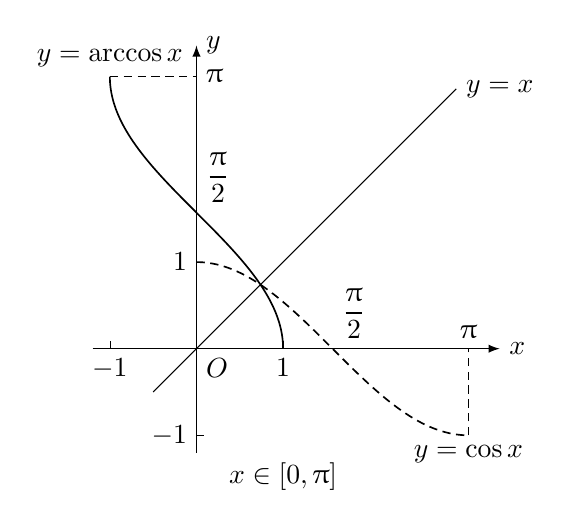
\begin{tikzpicture}[>=latex,scale=1.1]
  \draw[->](-1.2,0)--(3.5,0)node[right]{$x$};
  \draw[->](0,-1.2)--(0,3.5)node[right]{$y$};
  \node at (0,0)[below right]{$O$};
  \draw[semithick,samples=200,domain=0:pi] plot ({cos(\x r)},\x)node[above]{$y=\arccos x$};
  \draw[semithick,densely dashed,samples=200,domain=0:pi] plot (\x,{cos(\x r)})node[below]{$y=\cos x$};
  \draw(-0.5,-0.5)--(3,3)node[right]{$y=x$};
  \draw[densely dashed](-1,pi)--(0,pi)node[right]{$\uppi$};
  \draw[densely dashed](pi,-1)--(pi,0)node[above]{$\uppi$};
  \draw[very thin](-1,0)node[below]{$-1$}--++(0,0.09);
  \draw[very thin](1,0)node[below]{$1$}--++(0,0.09);
  \draw[very thin](0,-1)node[left]{$-1$}--++(0.09,0);
  \draw[very thin](0,1)node[left]{$1$}--++(0.09,0);
  \node at (1,-1.2)[below]{$x\in[0,\uppi]$};
  \node at (0,0.5*pi)[above right]{$\dfrac\uppi2$};
  \node at (0.5*pi,0)[above right]{$\dfrac\uppi2$};
\end{tikzpicture}
\end{document}